\section{创作者身份与未来：从“做视频”到“输出打动人心的作品”}

本章先给结论：Tim 在公司化之后重构身份的顺序，是把“创作者”放在最高位，再把管理者、艺人/表演者、产品经理这些角色放到创作使命之下。这个排序决定了他的未来叙事：公司要通过自由文化、本土化组织、持续迭代、商业模式升级和内部人才系统，长期输出能让人燃起来、能走向世界、能打动人心的作品。\footnote{源时间：01:11:02--01:17:44}

用教学化公式压缩这一章，可以写成：

$$
P_{\text{长期作品力}} = M \times I \times S \times B
$$

其中，$P_{\text{长期作品力}}$ 表示一家内容公司持续产出高价值作品的能力，$M$ 是使命方向，$I$ 是迭代速度，$S$ 是人才与组织系统，$B$ 是商业模式承载力。这个公式是本章的教学化概括，源视频没有提供数学公式。它提醒读者：创作者变成公司以后，真正被管理的对象已经扩展为愿景、人才、资源、技术和商业模式的组合。

\subsection{第一身份仍是创作者}

刘润在结尾处把问题问得很直接：现在怎么看待自己的定位，是创作者，还是老板。Tim 的回答也很直接：他认为自己第一身份仍然是创作者。他解释说，自己能带动团队，核心来自享受创作、把激情传递给别人，并且在开心时调动他人的共情；他主动降低了“高深管理术”在自我解释中的权重。\footnote{源时间：01:11:02--01:11:27}

\begin{dialoguebox}{身份排序的原话片段（源时间：01:11:02--01:11:57）}
\textbf{刘润}：你觉得你第一身份是个创作者，还是个老板？

\textbf{Tim}：我认为还是个创作者。本质上我也就是个做创作者的料。我是一个享受创作、能把激情传递给别人的人。

\textbf{Tim}：第一顺位还是创作者，第二顺位是管理者，第三顺位是艺人，第四顺位可能是产品经理。
\end{dialoguebox}

这段对话的教学价值在于，它把身份排序写成了组织设计的入口。第一身份是创作者，意味着公司愿景的源头仍然是作品；第二身份是管理者，说明作品需要团队、流程和结果约束；第三身份是艺人/表演者，说明 Tim 自己也承担镜头前的人格表达和情绪调动；第四身份是产品经理，说明“怪点子”需要落到产品、体验和商业承接上。

\begin{figure}[htbp]
  \centering
  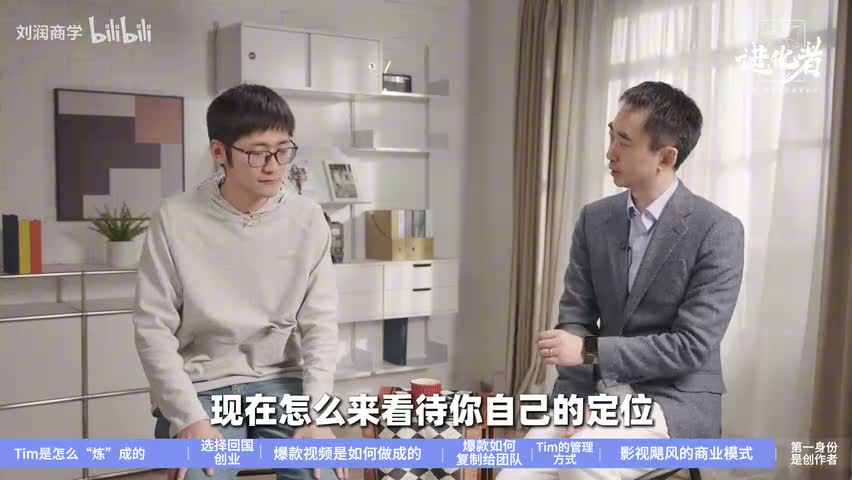
\includegraphics[width=0.70\linewidth,height=0.30\textheight,keepaspectratio]{figures/selected/frame_01-11-03_creator_identity_question.jpg}
  \caption{身份讨论的开场问题：创作者公司化以后，第一身份的排序会影响后续管理、商业与愿景选择。\protect\footnotemark}
  \label{fig:section06-creator-identity-question}
\end{figure}
\footnotetext{视频画面时间区间：01:11:00--01:11:06}

把这四个身份放在一起看，Tim 的角色结构更接近“创作型经营者”。创作者提供情绪燃料和作品判断，管理者把判断交给团队执行，艺人/表演者维持公众表达的感染力，产品经理把创意转换成可被使用、可被购买、可被反复优化的内容产品。前五章讲的是爆款、团队、OKR 和商业闭环；第六章把这些机制收束到一个问题：这家公司最后由什么价值观牵引。

\subsection{Netflix 参照：自由文化需要本土化落地}

刘润提到 Tim 过去说过，希望把自己做成一家像 Netflix 那样的公司。Tim 的解释很清楚：他好奇一家上万人规模的公司，怎样长期产出优质剧集；他认可 Netflix 过去创造了许多优秀内容，也学习其自由文化理念，同时强调不同国家、不同文化需要本土化适配。\footnote{源时间：01:11:57--01:12:37}

\begin{knowledgebox}{Netflix 自由文化在这里指什么}
本章把“Netflix 自由文化”理解为一种组织参照：尽量提高人才密度、给创作者更大自主权、用充分上下文和结果标准替代细碎过程管控。Tim 在访谈里没有展开制度细节，因此正文只使用源内明确出现的“自由文化”和“本土化适配”两个层面，不把外部管理理论强行套入影视飓风。
\end{knowledgebox}

这里的“本土化”很重要。自由文化如果直接照搬，容易变成口号；落在一家中国内容公司里，它必须回答更具体的问题：什么岗位可以高度自主，什么预算需要制片约束，什么内容需要 Tim 亲自过稿，什么 KR 能检验影响力，什么商业内容必须同时对甲方、创作者和观众负责。也就是说，Netflix 提供的是参照系，影视飓风要把它翻译成自己的组织语言。

从前文看，这种翻译已经有几层基础：第三章的编导、制片、专职人才与内容矩阵；第四章的自由化管理和 OKR；第五章的创意权、三方金字塔和平台风险。第六章的 Netflix 参照延续这些话题，回答一个更大的组织命题：创意公司扩张以后，怎样让自由继续服务作品质量。

\subsection{公司使命：无限进步与让中国人燃起来}

当刘润追问未来要把公司带到哪里，Tim 先回到一个经验：很多事情一开始听起来都很离谱，比如 2015 年说想有卫星，后来真的有了卫星。由此，他引出公司的座右铭“无限进步”：只有迭代能与残酷的世界抗争。\footnote{源时间：01:13:11--01:13:38}

\begin{importantbox}{使命、迭代与作品的关系（源时间：01:13:29--01:15:38）}
本章的核心关系可以概括为：使命给方向，迭代给抗压能力，技术和商业模式提供能力底座，作品承担最终的情绪与价值输出。若只保留“让中国人燃起来”这句口号，读者会丢掉机制；若把“无限进步”落实到技术、商业模式和人才系统，使命才有机会变成持续作品力。
\end{importantbox}

“让中国人燃起来”是 Tim 给出的公司使命。他解释这种“燃”来自少年时看热血动漫的感受，也来自对现实压力的观察：许多中国年轻人背负家庭期待、社会机会变化和成熟社会带来的疲惫感。影视飓风能做的事情有限，其中一个具体角色是做“小火花”，让观众看到世界上还有这样的活法、这样的内容，从而对明天多一点期待。\footnote{源时间：01:13:49--01:14:46}

这句话容易被读成鸡汤，所以必须把它拉回内容公司的工作台。“燃”在这里不能停留在单纯口号或宏大词汇里。它更像一种心理能量：观众看见不同活法、不同技术、不同冒险和不同作品后，眼里多一点光，心里多一点行动可能性。第二章的“共鸣”、第五章的“打动人心”，到这里被升级成公司的使命语言。

\begin{warningbox}{愿景最容易变成空口号}
“无限进步”“让中国人燃起来”“向世界输出打动人心的作品”都很大。大愿景一旦脱离机制，就会变成漂亮标语。检验方法很简单：它能否改变选题标准、预算分配、人才培养、技术投入、商业模式和复盘动作。能改变动作，愿景才进入组织；只能写在墙上，愿景就停留在修辞。
\end{warningbox}

\subsection{愿景：媒介会变，打动人心保持底层稳定}

Tim 接着把愿景推到更高一层：以不断迭代的技术和商业模式，向世界输出打动人心的作品。他特别强调，内容和商业模式同等重要，商业模式会随着科技和技术变化而变化；作品形态也会随着 VR、眼镜等媒介变化而变化，视频消费和内容消费方式可能随之改变，“打动人心”仍是底层稳定项。\footnote{源时间：01:14:49--01:15:38}

\begin{dialoguebox}{愿景的原话片段（源时间：01:14:49--01:15:38）}
\textbf{Tim}：以不断迭代的技术和商业模式，向世界输出打动人心的作品，这是我们的底层内核。

\textbf{Tim}：内容和商业模式是同等重要的。商业模式会随着科技和技术的变化产生变化。

\textbf{Tim}：作品形态会变化，随着 VR、眼镜上来，内容消费都会变化；打动人心是底层的。
\end{dialoguebox}

这段话把“内容理想”和“经营现实”接在一起。内容公司同时面对两条约束：作品缺少现金流会受限；商业模式消耗作品信用会伤害观众信任。Tim 选择把两者并列，说明他理解内容公司的底层矛盾：作品需要商业供血，商业需要作品信用，技术变化又会不断改写两者的连接方式。

\begin{figure}[htbp]
  \centering
  
\includegraphics[width=0.70\linewidth,height=0.30\textheight,keepaspectratio]{figures/selected/frame_01-15-05_content_business_equal.jpg}
  \caption{Tim 将内容与商业模式并列，提示读者：愿景要靠作品价值和经营结构共同承载。\protect\footnotemark}
  \label{fig:section06-content-business-equal}
\end{figure}
\footnotetext{视频画面时间区间：01:15:00--01:15:09}

VR、智能眼镜和新型显示设备只是例子。更普遍的规律是，媒介一变，叙事节奏、交互方式、成本结构、分发平台和商业模型都会跟着变。短视频改变了信息密度，直播改变了销售链路，VR 和眼镜可能改变沉浸感与第一视角表达。对影视飓风这样的公司来说，真正稳定项落在让观众产生情绪触动、价值认同和记忆点的能力上。

\begin{figure}[htbp]
  \centering
  
\includegraphics[width=0.82\linewidth,height=0.36\textheight,keepaspectratio]{figures/generated/fig_mission_iteration_work_relation.pdf}
  \caption{使命 / 迭代 / 作品关系图：使命给方向，迭代提供抗压能力，技术与商业模式支撑作品持续触达人心。图形综合自 01:13:33--01:15:30。}
  \label{fig:section06-mission-iteration-work-relation}
\end{figure}

图 \ref{fig:section06-mission-iteration-work-relation} 把这组关系压缩成一个循环：使命指向“让中国人燃起来”，方法是“无限进步/持续迭代”，能力底座来自技术和商业模式，输出是打动人心的作品；当观众对明天多一点期待，使命又获得新的反馈。这个循环解释了 Tim 谈未来时怎样从“做更大账号”推进到“向世界输出作品”。

\subsection{2028 奥斯卡目标：敢想，也要靠体系搭建}

最后，Tim 给出一个非常高的远期目标：2028 年希望拿到奥斯卡短片奖，或者戛纳、圣丹斯等重要电影节奖项；他强调希望是获奖，提名还不够。他也补充说，长片可能暂时够不到，短片有概率冲击。这一目标延续了早年“星辰大海和奥斯卡”的公司命名想象，也延续了从“放卫星”到真实卫星项目的敢想路径。\footnote{源时间：01:15:41--01:16:34}

这里需要冷静处理。奥斯卡和电影节奖项需要审美、工业、叙事、国际传播和评奖机制共同支撑，喊出目标无法自动缩短距离。Tim 的话真正有价值的部分，在于他马上把目标落回系统：自己未必亲自拍摄那部片子；他的责任是搭建体系，让公司内部有人能够站出来。\footnote{源时间：01:16:34--01:16:44}

这句话完成了从个人创作者到内容公司的身份转换。早期，Tim 是亲自写、亲自拍、亲自学、亲自更新的人；公司化以后，他还要让别人有机会站到作品中心。所谓体系，至少包括五件事：选题机制能发现高价值故事，制片机制能承载高难度项目，人才机制能让年轻创作者成长，商业机制能支付长期投入，文化机制能允许大胆目标出现。

结尾还提到两个未来计划：一个与“船”相关，另一个与太空相关；Tim 没有展开细节，只表示未来两三年可能会看到更有趣、更惊讶、更不可思议的事情。\footnote{源时间：01:16:46--01:17:19} 这些内容适合保留为方向性线索，不能写成已确定项目成果。对读者更重要的启发是：愿景型公司需要保留足够大的想象空间，同时用组织系统把想象转成可执行项目。

\subsection{本章小结}

本章把访谈的最后六分多钟收束成一个身份与愿景模型：Tim 的第一身份是创作者，第二身份是管理者，第三身份是艺人/表演者，第四身份是产品经理。这个排序说明，影视飓风的未来叙事依旧从作品出发，再通过管理、表达和产品化能力把作品放大。

\begin{itemize}
  \item 创作者身份提供源头判断：享受创作、传递激情、调动共情，是 Tim 解释自己能带动团队的核心原因。
  \item Netflix 提供组织参照：自由文化有启发意义，落地时需要本土化，必须被翻译成岗位、预算、目标、复盘和结果标准。
  \item “无限进步”给出方法论：只有持续迭代技术、流程、商业模式和人才系统，内容公司才有抗压能力。
  \item “让中国人燃起来”给出使命方向：作品要让观众看见不同活法，对明天多一点期待。
  \item “向世界输出打动人心的作品”给出长期愿景：媒介和商业模式会变化，触达人心的能力保持底层稳定。
  \item 2028 年奥斯卡短片或重要电影节目标给出远期牵引：真正关键的是搭建体系，让内部创作者能够站出来完成更高规格的作品。
\end{itemize}

至此，全片的主线完成闭环：从表达欲开始，经由爆款机制、团队复制、自由化管理、商业闭环，最后回到创作者使命。内容创业的终点从“把账号做大”升级为建立一个能持续产出好作品、能承受技术与商业变化、能让更多创作者向前站的系统。
